\documentclass{article}

\usepackage{fancyhdr}
\usepackage{extramarks}
\usepackage{amsmath}
\usepackage{amsthm}
\usepackage{amsfonts}
\usepackage{tikz}
\usepackage[plain]{algorithm}
\usepackage{algpseudocode}
\usepackage[encapsulated]{CJK}
\usepackage{graphicx}
\graphicspath{ {./images/} }

\usetikzlibrary{automata,positioning}

%
% Basic Document Settings
%

\topmargin=-0.45in
\evensidemargin=0in
\oddsidemargin=0in
\textwidth=6.5in
\textheight=9.0in
\headsep=0.25in

\linespread{1.1}

\pagestyle{fancy}
\lhead{\hmwkAuthorName}
\chead{\hmwkClass\:\hmwkTitle}
\rhead{\firstxmark}
\lfoot{\lastxmark}
\cfoot{\thepage}

\renewcommand\headrulewidth{0.4pt}
\renewcommand\footrulewidth{0.4pt}

\setlength\parindent{0pt}

%
% Create Problem Sections
%

\newcommand{\enterProblemHeader}[1]{
    \nobreak\extramarks{}{Problem \arabic{#1} continued on next page\ldots}\nobreak{}
    \nobreak\extramarks{Problem \arabic{#1} (continued)}{Problem \arabic{#1} continued on next page\ldots}\nobreak{}
}

\newcommand{\exitProblemHeader}[1]{
    \nobreak\extramarks{Problem \arabic{#1} (continued)}{Problem \arabic{#1} continued on next page\ldots}\nobreak{}
    \stepcounter{#1}
    \nobreak\extramarks{Problem \arabic{#1}}{}\nobreak{}
}

\setcounter{secnumdepth}{0}
\newcounter{partCounter}
\newcounter{homeworkProblemCounter}
\setcounter{homeworkProblemCounter}{1}
\nobreak\extramarks{Problem \arabic{homeworkProblemCounter}}{}\nobreak{}

%
% Homework Problem Environment
%
% This environment takes an optional argument. When given, it will adjust the
% problem counter. This is useful for when the problems given for your
% assignment aren't sequential. See the last 3 problems of this template for an
% example.
%
\newenvironment{homeworkProblem}[1][-1]{
    \ifnum#1>0
        \setcounter{homeworkProblemCounter}{#1}
    \fi
    \section{Problem \arabic{homeworkProblemCounter}}
    \setcounter{partCounter}{1}
    \enterProblemHeader{homeworkProblemCounter}
}{
    \exitProblemHeader{homeworkProblemCounter}
}

%
% Homework Details
%   - Title
%   - Due date
%   - Class
%   - Section/Time
%   - Instructor
%   - Author
%

\newcommand{\hmwkTitle}{Homework\ \#1}
%\newcommand{\hmwkDueDate}{September 17, 2015}
\newcommand{\hmwkClass}{Graph Theory}
\newcommand{\hmwkClassTime}{}
\newcommand{\hmwkClassInstructor}{}
\newcommand{\hmwkAuthorName}{Lin Hung Cheng B01902059}

%
% Title Page
%

\title{
    \vspace{2in}
    \textmd{\textbf{\hmwkClass:\ \hmwkTitle}}\\
    %\normalsize\vspace{0.1in}\small{Due\ on\ \hmwkDueDate\ at 3:10pm}\\
    %\vspace{0.1in}\large{\textit{\hmwkClassInstructor\ \hmwkClassTime}}
    \vspace{3in}
}

\author{\textbf{\hmwkAuthorName}}
\date{}

\renewcommand{\part}[1]{\textbf{\large Part \Alph{partCounter}}\stepcounter{partCounter}\\}

%
% Various Helper Commands
%

% Useful for algorithms
\newcommand{\alg}[1]{\textsc{\bfseries \footnotesize #1}}

% For derivatives
\newcommand{\deriv}[1]{\frac{\mathrm{d}}{\mathrm{d}x} (#1)}

% For partial derivatives
\newcommand{\pderiv}[2]{\frac{\partial}{\partial #1} (#2)}

% Integral dx
\newcommand{\dx}{\mathrm{d}x}

% Alias for the Solution section header
\newcommand{\solution}{\textbf{\large Solution}}

% Probability commands: Expectation, Variance, Covariance, Bias
\newcommand{\E}{\mathrm{E}}
\newcommand{\Var}{\mathrm{Var}}
\newcommand{\Cov}{\mathrm{Cov}}
\newcommand{\Bias}{\mathrm{Bias}}

\begin{document}

\maketitle

\pagebreak

\begin{homeworkProblem}
  \begin{CJK}{UTF8}{bsmi} % 開始 CJK 
    試證明, 假設把8 × 8的西洋棋盤上位於同一條對角線上的兩個頂角格子去掉 (於是剩下一個只有62 格的棋盤), 則這個棋盤沒辦法分割成若干個1 × 2 的長方形。並請利用同樣的論證描述在二分圖當中的一般性結論。\\

    \textbf{Solution}

    已知條件
    \begin{enumerate}
    \item 西洋棋盤上本有32個黑格子,32個白格子
    \item 同一條對角線上的兩個頂角格子必為同顏色
    \item 1 × 2的長方形當中,必然包含1個黑格子,1個白格子
    \end{enumerate}
    去除對角線上的兩個頂角格子後,只有兩種情形
    \begin{enumerate}
    \item 32個黑格子,30個白格子
    \item 30個黑格子,32個白格子
    \end{enumerate}
    必定無法將所有格子切割成1 × 2 的長方形
    \\
    \textbf{用二分圖證明}
\\可以將黑格子和白格子視為二分圖的兩部份,由於目標是分割成\(1\times2\),且各包含一個黑白格子的長方形,可以將目標視為在二分圖中,作1對1映射,即每個vertex的degree均為1。\\
    假設每個vertex的degree為1,在兩邊vertex數不同的情況下,則會發現兩部份的degree和不同,產生矛盾。
  \end{CJK}
\end{homeworkProblem}

\begin{homeworkProblem}
  \begin{CJK}{UTF8}{bsmi} % 開始 CJK 
    平面上有 n 個相異點, 已知任兩點的距離至少為 1。 試證明, 最多只有 3n 對點的距離恰為 1。 (提示:考慮將這些點距離恰為 1 者連邊。 請問在所給的條件之下, 每個點的度數至多為多少?)

    \textbf{Solution}
    \\
    取一點v,若要產生最多對點距離為1,則其neighbor \(v^1\) 和v的距離均為1,且\(v^1 \)中的點彼此有最多點距離為1。\\
    可以發現,\(v^1 \)中的點最多只能和2個其他\(v^1 \)中的點距離為1(可從v和\(v^1\)的其中一點畫出半徑為1的同心圓得知)。
    按照這個方法產生點,v最多會有6個neighbor,連邊之後會形成6個正三角形。\\
    所以n個點最多可以產生 \(n \times 6 \div 2 = 3n \)個點對距離為1。
  \end{CJK} % 結束 CJK 環境 
\end{homeworkProblem}

\pagebreak

\begin{homeworkProblem}
  \begin{CJK}{UTF8}{bsmi} % 開始 CJK 
    試證明, 腰圍為 5 的 k-正則圖至少有 $k^2 + 1$ 點。 對於 k = 2 或 3, 具體找出一個恰具有 $k^2 + 1$ 點的這種圖\\
    \textbf{graph of k = 2 or 3}
    \begin{figure}[h]
      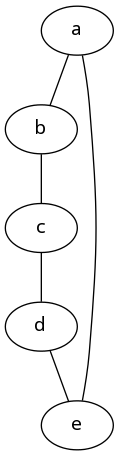
\includegraphics[scale=0.3]{graph1.png}
      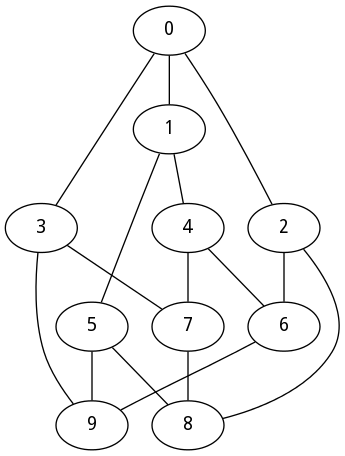
\includegraphics[scale=0.3]{graph2.png}
      \centering
    \end{figure}

    \proof
    在k-正則圖中取一個點v,其neighbor為 \(v^1 \),\(v^1 \)除了v之外的neighbor為\(v^2\)。\\
    可知 \(v^1  \bigcap  v^2  = \emptyset  \),否則會產生3-cycle(\(v - v^1_1 - v^2_1 - v\)),且 \(v^1 \)不會有v 以外的共同neighbor,否則會產生4-cycle(\(v - v^1_1 - v^2_1 - v^1_2 - v\))。\\
    因為是k正則圖,\(v^1 \) 有 \(k\) 個,\(v^2 \) 有 \(k(k-1)\) 個(每一個 \(v^1 \) 中的點的neighbor,除去v後有k-1個)。\\
    最少會有 \(1 + k + k(k-1) = k^2 + 1\) 個點
    % dot -Tpng graph1.dot -o graph1.png
  \end{CJK} % 結束 CJK 環境 
\end{homeworkProblem}

\begin{homeworkProblem}
  \begin{CJK}{UTF8}{bsmi} % 開始 CJK
    令圖 G 的點集是所有長度為 n 的二進位字串, 即 a1 a2 . . . an 、其中 ai ∈ {0, 1}。
    而兩個字串相鄰的條件是它們恰有兩個對應的位置不同。 試求 G 的連通部分的個數。\\
    \solution
    \\
    將兩個點的距離定義為字串對應位置不同的個數,可以發現連通部分中,任意兩個點的距離均會是偶數。\\
    令\(v_0 \)為 $ \{a_i = 0 |  i = 1\sim n\}$,可以分成兩個子集: \{和\(v_0\)距離為偶數的集合,和\(v_0\)距離為奇數的集合\}
  \end{CJK} % 結束 CJK 環境 
\end{homeworkProblem}

\begin{homeworkProblem}
  \begin{CJK}{UTF8}{bsmi} % 開始 CJK
    (a) 試證明, 圖 G 和其補圖 G 中至少有一個是連通的\\
    (b) 試證明, 若圖 G 是 P4-免除且非 K1 , 則 G 和 G 中有一個是不連通的
    \begin{proof}       
        
    (a)\\
    若圖G不連通,令G的連通部分為\(c_1, c_2, c_3 ... c_n\)。\\
    則補圖 \(\bar{G}\)會有\(c_1\)中所有點連到\(c_i(i = 2 ~ n)\)中的所有點,這會使\(\bar{G}\)連通。\\
    補圖G不連通的證明同理。\\
    (b)\\
    %已知圖G和其補圖至少有一個是連通的。\\
    因為\(P_4\)的補圖和\(P_4\)同構,所以\(\bar{G}\)也會是\(P_4\)-free,用G或\(\bar{G}\)來證明是相同的。\\
    %可以發現,若四個點的圖Q並非\(P_4\),Q 和 \(\bar{Q}\) 其中一個會是不連通的。

    若\(n = |V(G)|\),可列舉得知在 \(n \leq 3\) 的情況下會成立。\\
    設在\(n \geq 4\)的時候也成立。\\
    則在\(P_4-free, n \geq 4\)的連通圖G中,可找到一點V,使\(G'\) = G-V不連通(若在G中無此點,則考慮\(\bar{G}\)產生的\(\bar{G'} = \bar{G} - V\),證明方法相同,因為依照歸納法假設,\(G'\)和\(\bar{G'}\)有一個是不連通的。)\\
    若V與所有其他點相連,則\(\bar{G}\)不連通,若V不和\(G'\)相連,則\(G\)不連通。\\
    除此之外的相連方式,在\(G\)中,V和\(G'\)的至少兩個連通部分相連(若只連一個連通部分,則\(G\)會不連通)。其和V連結的其中兩個連通部分為\(c_1, c_2\),令V和\(c_1\)的neighbor為W,\(c_2\)的neighbor為Y。\\
    \(G'\)中也會存在一個與V不相鄰的點,令其為Z,在不失一般性的情況,可以令Y和Z相鄰。如此\(G\)中便存在 Z--Y--V--W 的 P4 導出子圖,矛盾。\\
    所以可能的情形只有V與所有其他點相連,而會使\(\bar{G}\)不連通。\\
    所以在\(P_4-free, n \geq 4\)的連通圖G中,\(G\)和\(\bar{G}\)有一個是不連通的。\\
    因為已證明\(n \leq 3\)也是成立,證明完成。\footnotemark
    \footnotetext[1]{參考資料: https://homepages.warwick.ac.uk/~masgax/Graph-Theory-notes.pdf}
  \end{proof}
\end{CJK} % 結束 CJK 環境 
\end{homeworkProblem}

\end{document}

%%% Local Variables:
%%% mode: latex
%%% TeX-master: t
%%% End:
